\subsection{Splay}
\frame{
  \frametitle{Splay?}
    \begin{columns}
      \begin{column}{0.4\textwidth}
        \begin{center}
          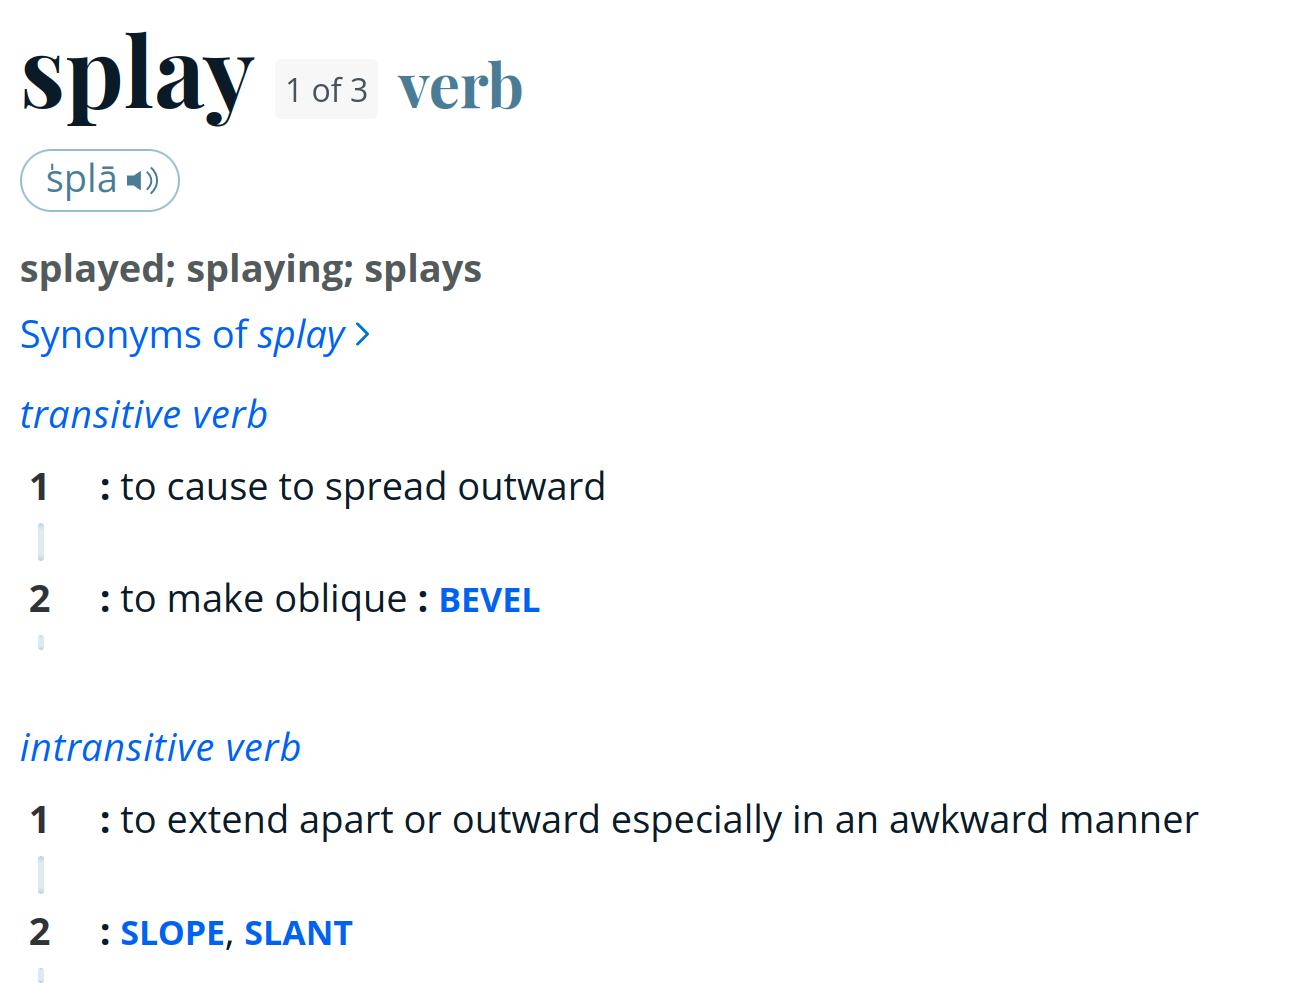
\includegraphics[width=\textwidth]{slides/alphabet_trees/splay_def.png}
        \end{center}
      \end{column}
        \begin{column}{0.6\textwidth}
            \begin{center}
                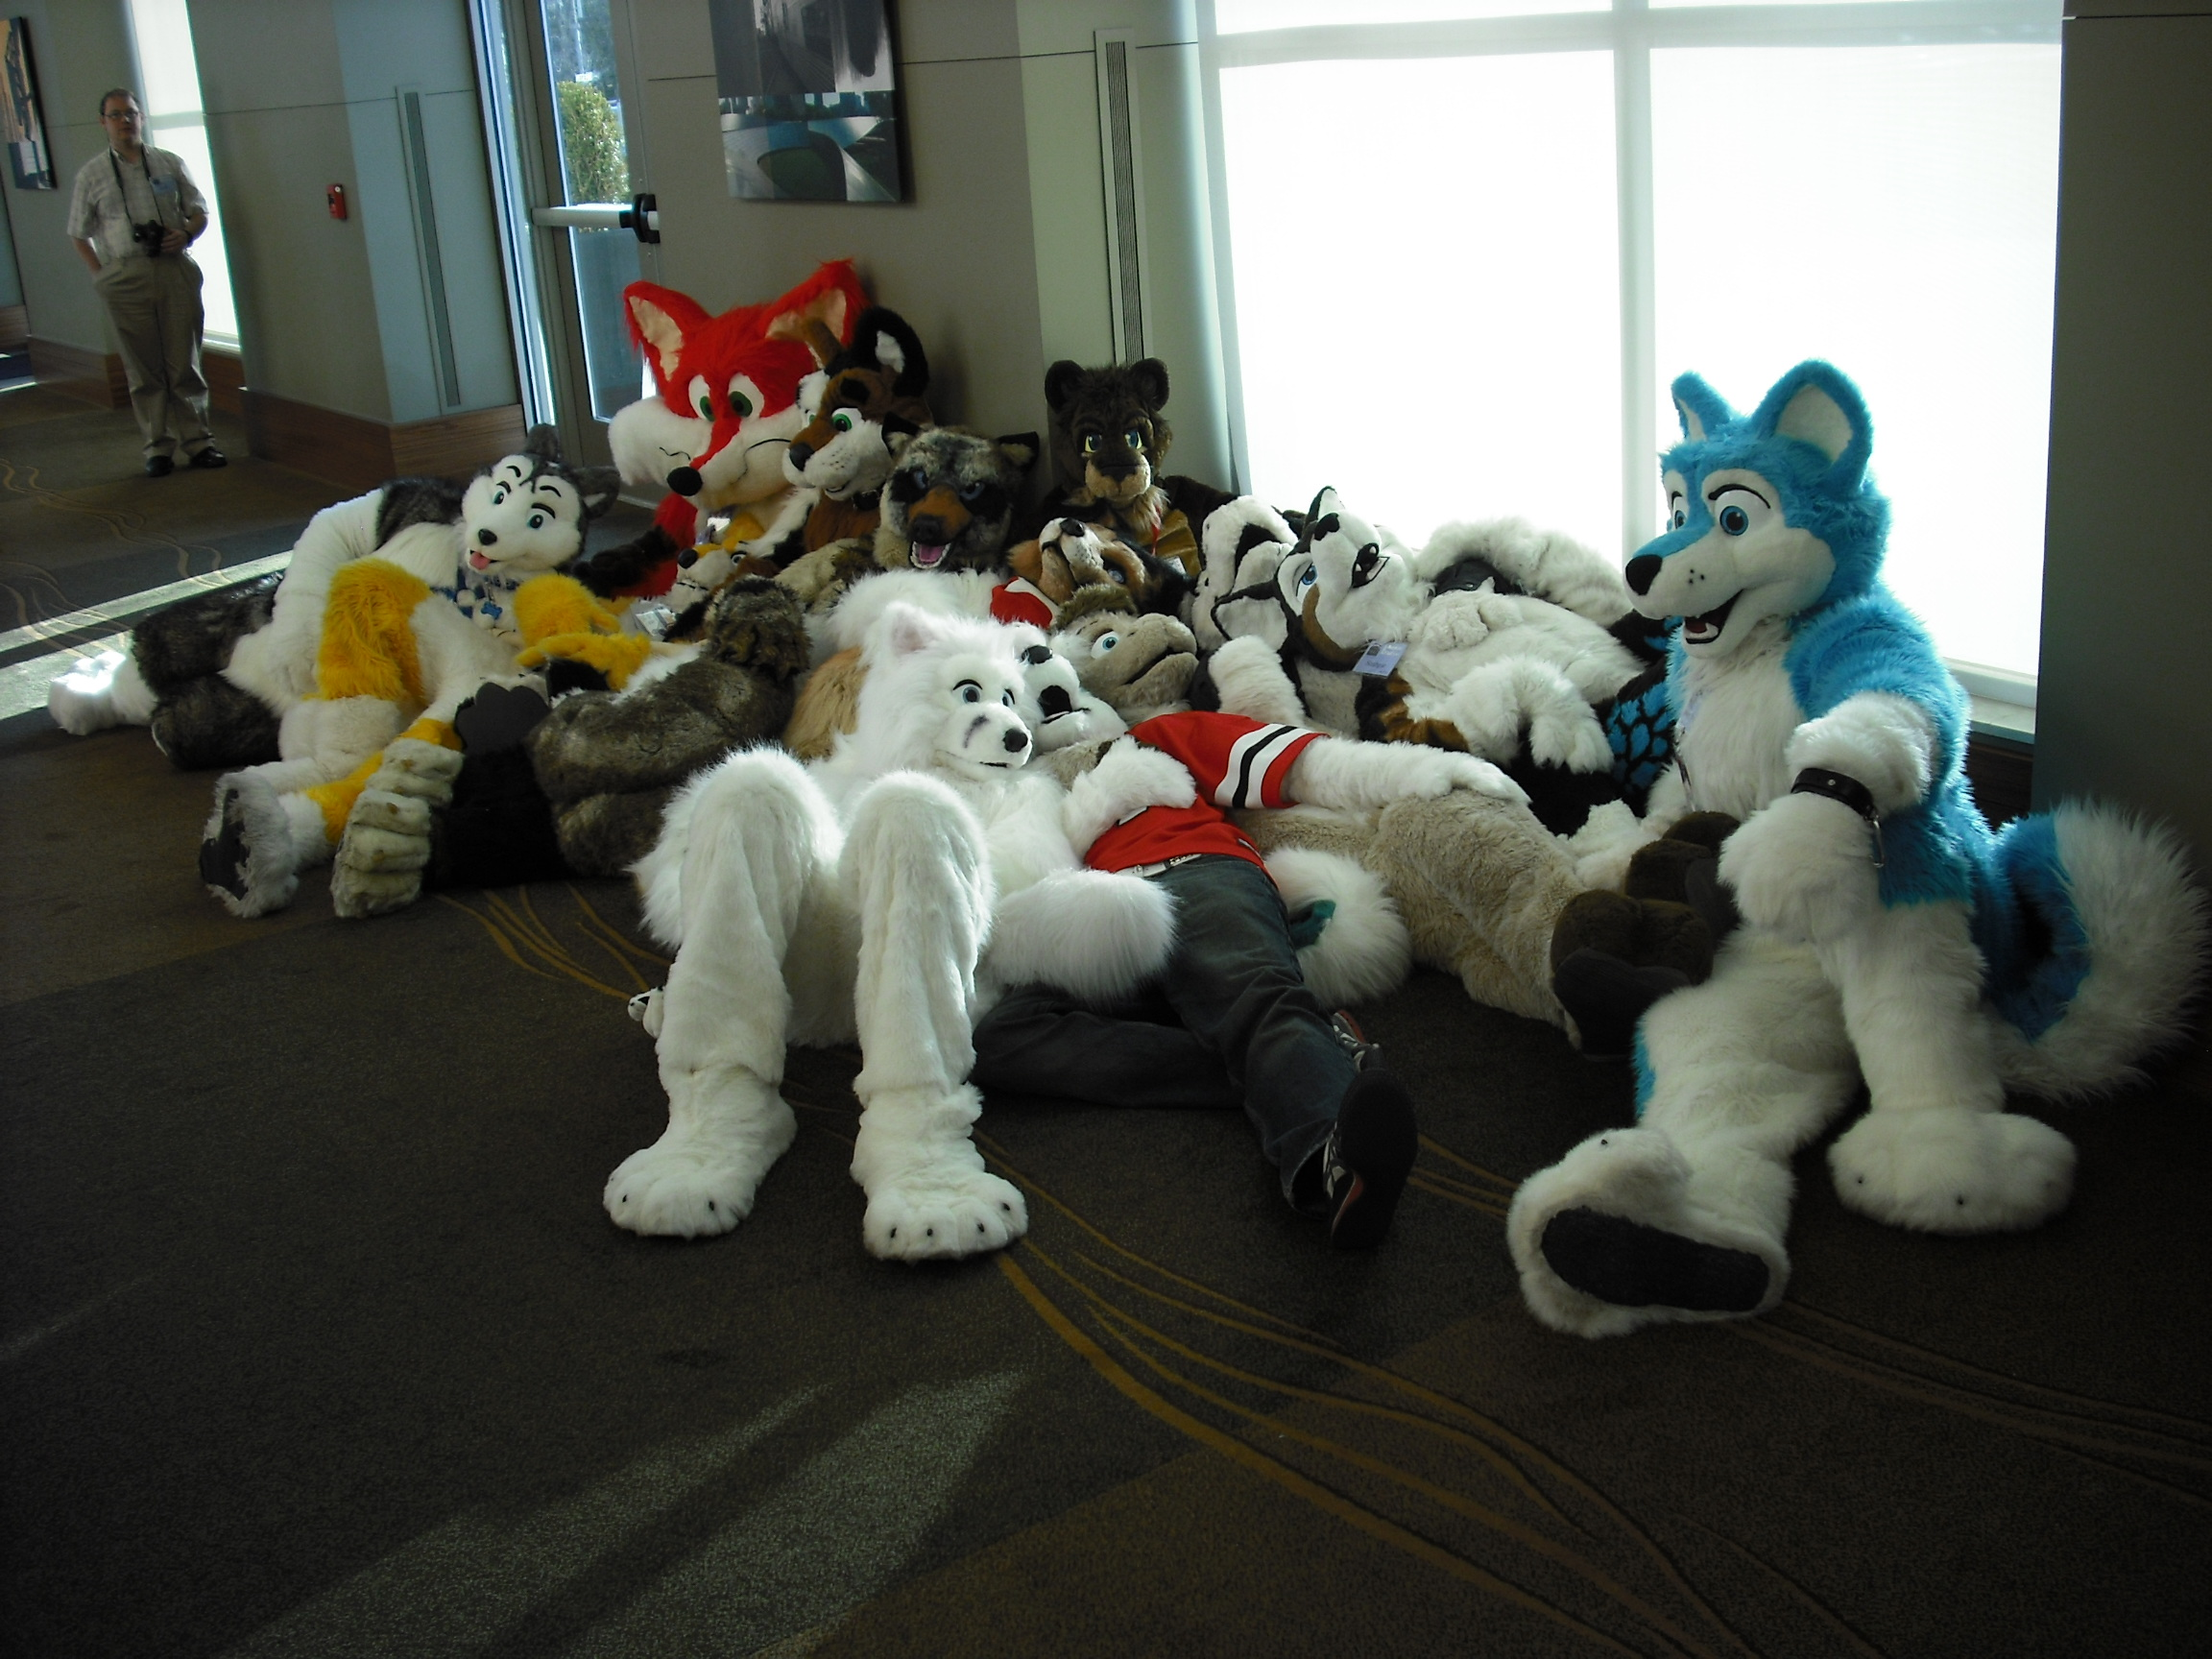
\includegraphics[scale=0.07]{slides/alphabet_trees/MFF2008_Furpile.JPG}

                {\tiny https://en.wikifur.com/wiki/Furpile}
            \end{center}
        \end{column}
  \end{columns}
}

\subsection{Splay Tree}
\frame{
  \frametitle{\subsecname\footnote{Sleator, Daniel D.; Tarjan, Robert E. (1985).}}
  \begin{columns}
      \begin{column}{0.5\textwidth}
          \begin{wideitemize}
            \item After every operation, splay the searched node to the root of the tree using double-rotations.
            \item Suspected to be optimal for any sequence of BST operations up to a constant factor (Dynamic Optimality Conjecture)
          \end{wideitemize}
      \end{column}
        \begin{column}{0.5\textwidth}
            \begin{center}
                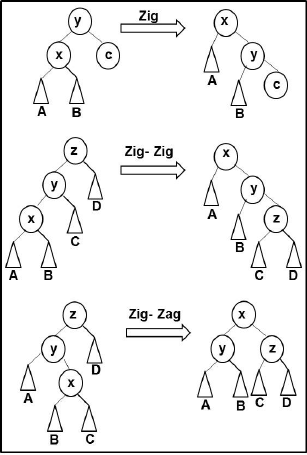
\includegraphics[scale=0.3]{slides/alphabet_trees/Splay-tree-basic-rotations-splaying-node-x-to-the-root.png}
                
                {\tiny \texttt{Trabelsi, Zouheir \& Zeidan, Safaa \& Masud, Mehedy \& Ghoudi, Kilani. (2015). Statistical Dynamic Splay Tree Filters.}}
            \end{center}
        \end{column}
  \end{columns}
}